\chapter{Software Design and Development}
\label{chap:software-design}

The work in this thesis uses the OpenMOC~\cite{openmoc} neutron transport code, which was developed for 2D \ac{MOC} simulations, to implement the 3D \ac{MOC} solver. Due to its strict focus on 2D simulations, great work was required to extend OpenMOC to 3D \ac{MOC} calculations. This chapter explains the structure of OpenMOC and the changes that were necessary to increase code flexibility in order to accommodate 3D \ac{MOC} calculations. 

This chapter begins with a general overview of OpenMOC in Section~\ref{sec:openmoc-overview}, with a focus on the Constructive Solid Geometry (CSG) representation of geometric detail. The interested reader can find a more complete description of the OpenMOC code in Boyd's thesis~\cite{boyd2014openmoc}. Next, the object oriented design is discussed in greater detail in Section~\ref{sec:object-oriented} with a focus on the changes to accommodate both 2D and 3D simulations. This discussion is continued in Section~\ref{sec:modular-structure}, where the new modular structure of OpenMOC is discussed as well as its importance in creating a robust simulation tool capable of supporting various algorithms. Section~\ref{sec:software-performance-considerations} discusses performance considerations in developing an efficient \ac{MOC} solver. In Section~\ref{sec:user-input} the standard Python user input is discussed as well as the new C++ alternative build which is attractive for \ac{HPC} applications where the availability of software required for the Python interface may be limited. Section~\ref{sec:version-control} concludes the chapter with a discussion of development practices and the open source license.

%%%%%%%%%%%%%%%%%%%%%%%%%%%%%%%%%%%%%%%%%%%%%%%%%%%%%%%%%%%%%%%%%%%%%%%%%%%%%%%%
\section{OpenMOC Overview}
\label{sec:openmoc-overview}

OpenMOC is neutron transport code that is written in C++ with a \ac{SWIG}~\cite{swig} to expose the C++ classes and routines to the Python scripting language. This allows users to take advantage of the simplicity and flexibility of the Python language while also having the performance benefits of C++ compiled code. In this way, users can work entirely in Python without having to touch the underlying C++ code. In addition, users do not have to learn a new input file syntax, only the names, functionality, and input variables of functions constituting the \ac{API}. This allows for users to write more natural code.

The underlying C++ code of OpenMOC also leverages the use of OpenMP~\cite{openmp} for shared memory parallelism. In this framework, all on-node data is shared between threads. With the emergence of the 3D solver, distributed parallelism has also been implemented with MPI~\cite{mpi} in the form of domain decomposition, discussed in Chapter~\ref{chap:domain-decomposition}. With this hybrid parallelism design, OpenMOC is able to scale to both many CPU cores and many nodes. 

OpenMOC is built on the use of \ac{CSG}, which allows complex geometries to be built out of boolean operations -- such as intersections and unions -- of simple surfaces and building blocks termed \textit{primitives}. In addition, a hierarchy is used to agglomerate collections of primitives together. This approach is particularly useful for reactor geometries which are often highly structured. For example, a typical reactor core is built out of simple \textit{fuel pins}, grouped together into \textit{assemblies}. Fuel pins describe the radial detail of a fuel rod. Assemblies are then grouped together to form the reactor core. An example of a 2D \ac{CSG} construction of a single assembly is given in Figure~\ref{fig:core-csg}.

\begin{figure}[h!]
	\centering
	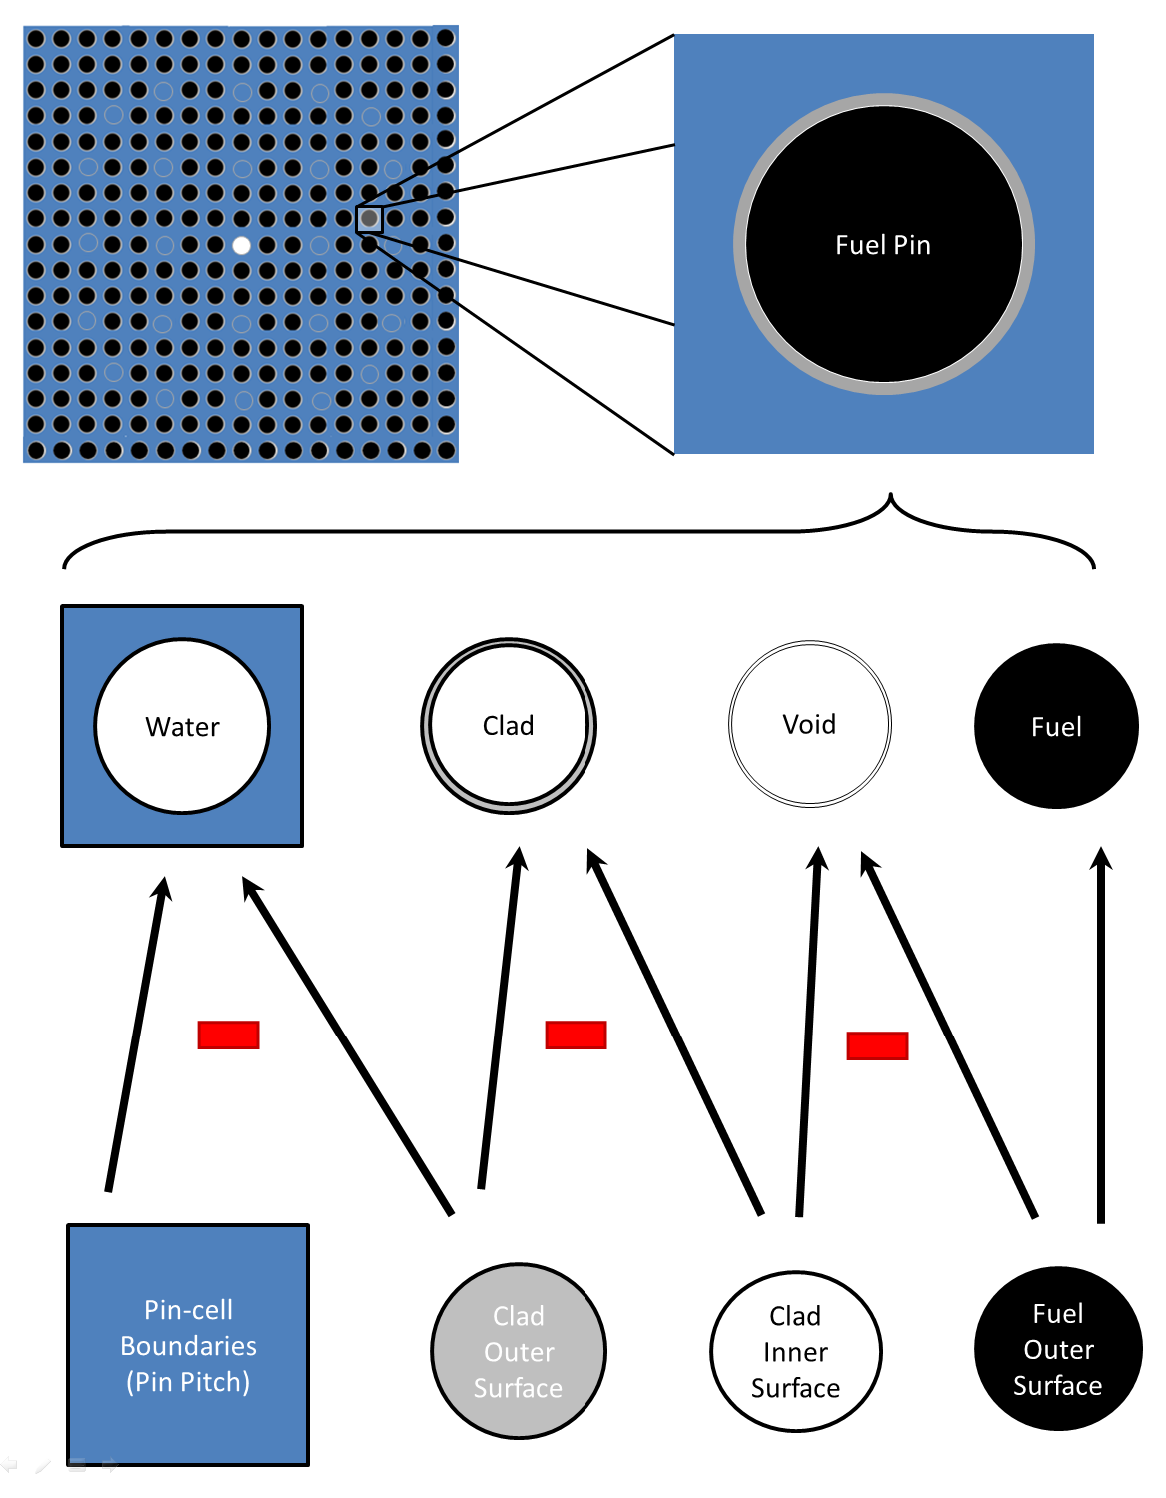
\includegraphics[width=0.9\linewidth]{figures/assembly-csg.PNG}
	\caption[]{The hierarchical CSG construction of a typical assembly.}
	\label{fig:core-csg}
\end{figure}

One of the benefits of the \ac{CSG} approach is a reduced memory requirements of storing the geometry. Instead of explicitly storing the geometry information of each fuel pin within the reactor core, only unique fuel pin types need to be stored. They are then referenced by their parent structure. For instance, an assembly containing a lattice of fuel pins creates a mapping of lattice location to the unique fuel pin type, rather than replicating the full geometric information for each fuel pin.

In addition, the formation of a \ac{CSG} allows ray tracing to be conducted in a general framework, agnostic of the individual primitives. Each \textit{cell} in OpenMOC is defined in terms of of \textit{surface} objects and the half-space of each surface. A half-space determines on which side of the surface the cell is located. Ray tracing fundamentally involves calculating the distance to intersection along a direction. With the \ac{CSG} framework, each of the bounding surfaces is queried for the distance to intersection. This naturally speeds up ray tracing by not having to check each instance of a surface within the geometry, but rather only the local surfaces. 

Once the geometry is built, OpenMOC generates tracks across the constructed geometry, and solves the neutron transport equation iteratively, as described in Chapter~\ref{chap:moc}. CMFD acceleration can also be included by the user, which utilizes the methods described in Chapter~\ref{chap:cmfd}.

Once the neutron transport equation is solved, the solver can be queried to return the scalar flux distribution as well as reaction rates. In order to visualize the data, OpenMOC includes Python plotting routines for scalar flux data, computed reaction rates, as well as geometric detail and visual diagnostics. 


%%%%%%%%%%%%%%%%%%%%%%%%%%%%%%%%%%%%%%%%%%%%%%%%%%%%%%%%%%%%%%%%%%%%%%%%%%%%%%%%
\section{Object Oriented Design}
\label{sec:object-oriented}

OpenMOC uses the object oriented programming paradigm whereby data structures called \textit{classes} are created that encapsulate both the data and associated subroutines. Object oriented programming generally leads to more resilient code since only the class itself can access its private attributes. An instantiation of a class is termed an \textit{object}. OpenMOC applies many of the principles of object oriented programming including information hiding, inheritance, and polymorphism.

An OpenMOC simulation requires three main components: a geometry, a track generator, and a solver. All of these are C++ classes in OpenMOC and exposed to the user. The user first describes the surfaces, cells, universes, and materials which constitute the geometry in a hierarchical \ac{CSG} arrangement. The user then instantiates a \texttt{Geometry} object and provides it the root cell of the \ac{CSG}. Next, a \texttt{TrackGenerator} is instantiated which is provided the \texttt{Geometry} object as well as track generation parameters such as radial ray spacing and number of azimuthal angles. Lastly, a \texttt{Solver} object is instantiated and provided the \texttt{TrackGenerator} object along with solver criteria such as the tolerance. The solver can then be called to solve the \ac{MOC} equations, such as the \ac{MOC} neutron transport eigenvalue problem, using the track and segmentation information found in the \texttt{TrackGenerator}.

Extending the OpenMOC solver to 3D simulations required restructuring all of these classes in order to make them more flexible. A focus in extending the sovler to 3D simulations was to still maintain the ability to run 2D simulations. A benefit of maintaining the ability to run 2D simulations is to allow the user to compare 2D and 3D simulations on the same problem. To accommodate this, the input structure between 2D and 3D simulations is very similar. In order to make the code more resilient and simpler, common code reuse was emphasized. Many of the routines present in the 2D simulations are also used in the 3D simulations so both should use the same code without re-writing those entire sections. These points illustrate the need for maximum cohesion between the 2D and 3D solver modes. This is accomplished by expanding the 2D classes to be more general.

\subsection{\texttt{Geometry} Class Updates}
\label{sec:oo-geometry}

The \texttt{Geometry} class was altered to accommodate piecewise \textit{axially extruded geometries}. Axially extruded geometries are geometric configurations in which the geometry looks the same at every axial level. A piecewise axially extruded geometry is a geometry that can be formed as the union of a finite number of extruded geometries. For instance, a fuel rod with end caps would fit the description of a piecewise axially extruded geometry but a sphere would not. Most practical reactor applications are indeed piecewise extruded geometries so this is not a very strong limitation. 

With the change from 2D geometries to piecewise axially extruded geometries, circles are transformed to $z$-cylinders (cylinders with a vertical major axis) and $z$-planes are added with a similar structure to the $x$ and $y$ planes already incorporated in OpenMOC. With this new geometry paradigm, 2D problems are thought of as simulating a radial slice of a 3D geometry at a given $z$ height. 

\subsection{\texttt{TrackGenerator} Class Updates}
\label{sec:oo-trackgenerator}

The \texttt{TrackGenerator} class was updated to generate tracks and ray trace, compatible with the updated \texttt{Geometry} class. 2D ray tracing is imagined as ray tracing tracing perpendicular to the $z$-axis at some $z$-height. By default this height is assumed to be 0.0 in order to limit the complexity of user input for 2D simulations. The user can specify a different $z$-height using the \texttt{setZCoord} function of the \texttt{TrackGenerator} class.

For 3D simulations, a new \texttt{TrackGenerator3D} class was created which inherits from the \texttt{TrackGenerator} class. In object oriented programming, a class that inherits from a parent class has access to all the parent class data and subroutines. Since tracks are built on a 2D projection, the 3D track generator must have all the functionality of the regular 2D track generator. This is the typical paradigm where class inheritance is useful. 

During ray tracing, a \texttt{TrackGenerator3D} object first ray traces all 2D tracks (determined from the parent \texttt{TrackGenerator} functionality) over all potentially unique $z$-planes in the geometry to form the equivalent of a ray trace over the composite of all radial detail in the geometry. Since this can potentially be expensive, users are allowed to indicate the unique piecewise axially extruded ranges in the \texttt{Geometry} through the \texttt{setSegmentationZones} function in the \texttt{TrackGenerator3D} class. If these zones are not specified, all $z$-planes in the geometry are viewed as a potential divider between different axially extruded regions.

Once the 2D ray trace is conducted over all axially extruded regions, the full 3D ray trace can be calculated. Due to the expense of explicitly storing all 3D tracks in a typical geometry, the \texttt{TrackGenerator3D} class generates tracks on-the-fly. Similarly, segments can be prohibitively expensive to store. Therefore, the default mode is to calculate segments on-the-fly rather than upfront, although both options are available. Ray tracing and segmentation is discussed in greater detail in Chapter~\ref{chap:ray-tracing}.

\subsection{\texttt{Solver} Class Updates}
\label{sec:oo-solver}

The \texttt{Solver} class has also been reformulated to support both 2D and 3D simulations. The \texttt{Solver} class is an abstract class, meaning it contains the description of data and associated subroutines, but cannot be instantiated on its own. Instead, there are subclasses that inherit from the abstract class that can be instantiated. In this case the \texttt{CPUSolver} and \texttt{GPUSolver} classes are both subclasses of the \texttt{Solver} class. Rather than supporting both the \texttt{CPUSolver} and \texttt{GPUSolver} classes, this thesis focuses on the \texttt{CPUSolver} class to allow for easier implementation of the object oriented structures.

The \texttt{CPUSolver} was altered to support the calculation of both 2D \ac{MOC} and 3D \ac{MOC} equations. By referring to the supplied \texttt{TrackGenerator} object, it can determine whether a 2D or 3D simulation should be calculated. If a \texttt{TrackGenerator3D} object was provided to the solver, it runs a 3D simulation. Otherwise, a 2D simulation is run. While much of the code is shared between the 2D and 3D simulations in the solver, the core code which calculates the variation of angular flux over segments has separate 2D \ac{MOC} and 3D \ac{MOC} code sections in order to maximize performance.

In addition to the existing \texttt{CPUSolver}, a new \texttt{CPULSSolver} class has been added to OpenMOC which is capable of using a linear source approximation. Since the linear source solver needs much of the code present in the regular flat source solver, \texttt{CPULSSolver} was implemented as a subclass of \texttt{CPUSolver}.

%%%%%%%%%%%%%%%%%%%%%%%%%%%%%%%%%%%%%%%%%%%%%%%%%%%%%%%%%%%%%%%%%%%%%%%%%%%%%%%%
\section{Modular Structure}
\label{sec:modular-structure}

In altering OpenMOC to support both 2D and 3D simulations, it was quickly realized that without a massive overhaul, there would be a very large amount of repeated code. The goal was to create code that was capable of conducting both 2D and 3D \ac{MOC} simulations, but also compare multiple types of ray tracing and mathematical approximations (such as linear source). For all these options to be supported, there is the possibility for much of the same functionality to be implemented at multiple points in the code.

For example, \ac{MOC} can largely be described as an algorithm that performs a ray trace and then computes equations over the segments formed from the ray trace. Many different ray tracing algorithms could be used with the underlying equations and solver remaining theoretically unchanged. However, if the code is rigid, each new ray tracing algorithm would require an entire code re-write.

Therefore, a goal in developing OpenMOC to support work presented in this thesis is to maximize code reuse. This not only shortens the code but also makes it more robust as algorithms tend to change frequently to update functionality and fix bugs. If code is repeated, it is likely that not all of the code would receive the appropriate updates. Additionally, comparing options in the code, such as ray tracing, becomes much more robust when the code run during comparisons only differs minimally with most of the differences being those directly tested.

A structure was created in which segment traversal, ray tracing, and the algorithms that use segment information could be easily decoupled. In this new structure, \texttt{MOCKernel} classes dictate what operations to perform on each segment and a \texttt{TraverseSegments} class dictates how to iterate over segments and which ray tracing method to use. Both of these classes are virtual classes which have subclass implementations. Specific algorithms that use segment information are formed as subclasses of the \texttt{TraverseSegments} class, each defining operations to perform on groups of segments. The algorithms should also specify which \texttt{MOCKernel} objects to use.

\subsection{\texttt{MOCKernel} Classes}

Since the \texttt{MOCKernel} class operates directly on segments, it appears in the inner-most loop in algorithms. The \texttt{MOCKernel} parent class contains common information used for most of its subclass implementations. These attributes include:
\begin{itemize}
	\item A counter for the number of segments encountered by the kernel
	\item The maximum path length allowed for segments before they must be split
	\item The number of energy groups
\end{itemize}

An \texttt{MOCKernel} class also has a few virtual functions that must be implemented by subclasses. Notable functions include:
\begin{itemize}
	\item An \texttt{execute} function which dictates what to do on a segment
	\item A \texttt{newTrack} function that dictates functionality when a new group of segments is encountered.
\end{itemize}
The \texttt{execute} function is applied immediately when a segment is formed from ray tracing (or loaded in the case of explicitly stored segments) whereas the \texttt{newTrack} function is applied at the start of sequencing through a group of segments. The segments comprising a track is an example of a common grouping of segments, though other groupings could be chosen.

Since the \texttt{MOCKernel} class is a virtual class, it is meant to have subclasses which can be instantiated. The current \texttt{MOCKernel} subclasses implemented in OpenMOC are:
\begin{itemize}
	\item \texttt{CounterKernel}: Counts the number of segments encountered by the kernel
	\item \texttt{VolumeKernel}: Uses track weights and segment lengths to form an estimate of the volumes of regions encountered
	\item \texttt{TransportKernel}: Directly applies the transport equation on the encountered segments
	\item \texttt{SegmentationKernel}: Caches segment information for use in later calculations
\end{itemize}
Since the \texttt{SegmentationKernel} object just caches information it is useful for complicated operations or operations which can be most efficient when applied to a bulk grouping of data. For this efficiency reason, the \texttt{TransportKernel} is not currently used in the default solver. Instead, a \texttt{SegmentationKernel} is used in its place so that the operations can be applied to flux data at once instead of interleaving ray tracing with transport calculations.

\subsection{\texttt{TraverseSegments} Classes}

Unlike the \texttt{MOCKernel} parent class, the \texttt{TraverseSegments} virtual class contains a significant amount of algorithmic information. Specifically, the virtual class contains all segment iteration and ray tracing algorithms. The algorithm has a \texttt{loopOverTracks} function that takes an \texttt{MOCKernel} as an argument. Subclasses of \texttt{TraverseSegments} can call this function which iterates over groups of segments (eg. tracks). 

Inside the \texttt{loopOverTracks} function, a conditional block calls the appropriate segment looping scheme, passing along the provided kernel. The currently implemented segment iteration schemes are:
\begin{itemize}
	\item \texttt{loopOverTracks2D}: Iteration scheme for looping over explicitly stored 2D segments
	\item \texttt{loopOverTracks3DExplicit}: Iteration scheme for looping over explicitly stored 3D segments
	\item \texttt{loopOverTracksByTrackOTF}: Iteration scheme for looping over and generating segments on-the-fly where segments in a track are looped over in order before switching to the next track
	\item \texttt{loopOverTracksByStackOTF}: Iteration scheme for looping over and generating segments on-the-fly where segments in a $z$-stack of tracks are looped over in order before switching to the next $z$-stack
\end{itemize}
Each of the iteration schemes loops over all tracks and segments in the problem in some order, performing the associated ray tracing algorithm when appropriate. The ray tracing scheme is provided information relevant to ray tracing or loading the segments of interest. In most cases, this pertains to all segments in a track. However, for the \texttt{loopOverTracksByStackOTF} scheme, all segments in a $z$-stack are traced at once. Before calling the ray tracing scheme, the \texttt{newTrack} function of the provided kernel is called. Then the ray tracing scheme is called and provided the kernel so that it can call the \texttt{execute} function immediately when the segment is formed or loaded. 

After the ray tracing scheme is completed, an \texttt{onTrack} function is called which details operations to perform on the group of segments. The cached segment information is also provided if a \texttt{SegmentationKernel} was used. The transport sweep algorithm currently used in OpenMOC applies all of the \ac{MOC} equations inside the \texttt{onTrack} function using the provided cached segment information.

In general, algorithms which require track or segment information should form a small subclass of the \texttt{TraverseSegments} function and define the \texttt{onTrack} function. Additionally, an \texttt{execute} function should be defined which details the general structure of the algorithm. It should include the setup, call the \texttt{loopOverTracks} function to loop over all segments and apply the algorithm defined by the \texttt{onTrack} function and the provided kernel, and then detail any operations to perform after looping over all tracks and segments. 

An example of an execute function is given below for the \texttt{VolumeCalculator} class which calculates the volumes of all regions in the geometry. Since it performs all operations directly on segments using \texttt{VolumeKernel} objects, the \texttt{onTrack} function is defined to simply return.

\begin{center}
\begin{lstlisting}
void VolumeCalculator::execute() {
	#pragma omp parallel
	{
		MOCKernel* kernel = getKernel<VolumeKernel>();
		loopOverTracks(kernel);
	}
}
\end{lstlisting}
\end{center}

For algorithms in which only operations need to be performed on tracks, a \texttt{NULL} kernel can be provided which alerts the segment iteration scheme to skip the ray tracing step. Numerous subclasses of \texttt{TraverseSegments} are present in OpenMOC since every algorithm which loops over segments or tracks is contained in a subclass of \texttt{TraverseSegments}. They all appear in the files \texttt{TrackTraversingAlgorithms.h} and \texttt{TrackTraversingAlgorithms.cpp}.

%%%%%%%%%%%%%%%%%%%%%%%%%%%%%%%%%%%%%%%%%%%%%%%%%%%%%%%%%%%%%%%%%%%%%%%%%%%%%%%%
\section{Performance Considerations}
\label{sec:software-performance-considerations}

So far this chapter has emphasized software design for code resiliency and flexibility. However, a useful application should also minimize runtime. This section concentrates on software design considerations to maximize performance and minimize runtime.

\subsection{Addressing Performance in Object-Oriented Modular Software Design}

While the object-oriented and modular design is useful for code reuse, minimizing the number of potential bugs and allowing for greater flexibility, it does add some computational overhead. The overhead is largely due to added function calls. This can be overcome through the use of \textit{inline functions} which inject their code directly into sections where they are called at compile time. While this increases the performance of the code, it can radically increase the size of the executable, especially for large inline functions. Therefore, functions should only be inline functions if they are small. For instance, inline functions are used in OpenMOC for computing surface intersections and tallying current to CMFD surfaces. 

However, successfully using inline functions can sometimes be difficult where logic is required to determine which function to call. Therefore, performance-sensitive code should be designed such that the number of function calls which are not inline functions are minimized.

The optimal code design blends object oriented and modular design for code that is not performance-critical while using optimized and less flexible code for the performance-sensitive sections. In terms of the \ac{MOC} algorithm, over 95\% of the runtime is typically spent applying the \ac{MOC} equations for a given segment. In OpenMOC, the application of the \ac{MOC} equations occurs in the \texttt{CPUSolver::tallyScalarFlux} function. This function, which is quite small in size, should be thoroughly optimized for performance while the rest of the code should rely heavily on object oriented and modular design principles. 

\subsection{Organizing Data Contiguously in Energy Groups}

One critical consideration when designing performance-sensitive code is the memory layout. When CPU cores load information from memory, they load entire cache lines into local caches rather than just the desired variable. This allows the number of loads to be reduced if nearby memory is accessed. When desired memory is already within the cache of the CPU core, it is termed a \textit{cache hit}. If it is not, it is termed a \textit{cache miss}, requiring an extra load. Optimizing cache performance to maximize cache hits is critical when designing efficient software, as loads from main memory can be quite expensive. \textit{Locality} refers to how well memory is organized such that nearby or local memory is accessed frequently. 

To maximize locality in \ac{MOC} applications, the data should be structured to be contiguous in energy groups. Generally, the \ac{MOC} equations can be approached as being applied to segments over several energy groups. Since \ac{MOC} tracks traverse regions in different orderings, it is difficult to optimize the cache efficiency of data accessed by region. However, the data for each region can easily be structured and always traversed in the same ordering. Therefore, the maximal amount of work should be completed on each region before moving to the next. This implies that the energy groups should all be treated together and the data structures should be contiguous in energy groups to reflect this memory access pattern. 

\subsection{Scratch Pads for Temporary Storage}

There are several points throughout the \ac{MOC} algorithm where quantities need to be temporarily stored by region or by group. One example is calculating total reaction rates. To compute a total reaction rate in the reactor, the reaction rates from all regions and energy groups need to be calculated and summed. It is possible to add each contribution from a region and group to a tally for the total reaction rate immediately after calculation, but this can lead to significant roundoff error. Alternatively, if the summed values could be first stored in an array and then added in a pair-wise fashion, the roundoff error can be significantly reduced.

The number of summed quantities is $NG$ where $N$ is the number of source regions and $G$ is the number of energy groups. An array of $NG$ could be allocated, but this would require a significant amount of additional storage. Instead, two arrays are allocated -- one of size $G$ and another of size $N$. Reaction rates for all $G$ groups for an individual region are computed and then stored in a temporary array of size $G$. This array is then summed using a pairwise sum. The result is then stored in an array of size $N$. After this conducted for all $N$ regions, the array of size $N$ is then summed in a pairwise fashion.

Since temporary arrays of size $N$ and size $G$ are often found throughout OpenMOC, memory for these arrays is allocated at the beginning of the solver for each thread. Allocating memory can often be quite costly. If the arrays were allocated just before use, there would be a significant number of memory allocations. By allocating the memory up front and later referencing the allocated memory, the number of memory allocations is minimized, improving performance.

\subsection{Minimizing Parallel Contention}

When multiple threads modify shared data, bugs can be incurred due to race conditions where the outcome of a program is dependent on the order in which threads execute operations. For instance, consider multiple threads adding numbers to a shared counter. The fundamental operations that access the data are reads and writes. Therefore, one thread could read a value of the counter and before the thread adds the read value with its added value, the counter updates. The thread then writes the computed value to the shared counter, disregarding the update that occurred after the read, leading to an error in the computation. This occurs because the read, addition, and write are separate operations where the data can be modified between the operations~\cite{shavit}.

Because of these considerations, care must be taken to ensure correctness in multi-threaded applications. A common way to ensure correctness is to place a \textit{lock} around \textit{critical sections}. A critical section is where shared data is potentially modified by multiple threads. A lock ensures that at most one thread can access the critical section at any time. While locks do ensure correctness, they can also cause a bottleneck in the code, especially when many threads are present and attempting to access the same critical section. This situation is termed \textit{contention}.

In terms of the \ac{MOC} algorithm, in which each thread is responsible for applying the \ac{MOC} equations to a group of segments, threads can be handling segments which access and modify data (such as the scalar flux) for the same region. A naive implementation would place a lock around the modification of the local scalar flux data for each energy group when the segment's contribution is computed. While this ensures correctness, it requires that each thread attempt to acquire a lock for each energy group, which can incur significant overhead cost.

Instead, each thread tallies the contributions to each energy group in its local temporary storage array, as mentioned in the previous section. This allows for the thread to modify the array without any contention with other threads. After the contributions are computed and stored for every energy group, a lock is acquired for the region and the local thread contributions are summed to the global tally of scalar flux. This allows for only one lock to be acquired for each segment traversal. In addition, it allows for increased cache efficiency and vectorization. Lock operations require much communication between cache levels to ensure correctness and are not vectorizable. By decreasing the frequency to which locks are accessed, these issues can be minimized.

\subsection{Computing Exponentials}

One major bottleneck of \ac{MOC} solvers, particularly for flat source \ac{MOC}, is the computation of exponentials. Since an exponential term is present in the \ac{MOC} equations, dependent on optical path length, an exponential needs to be computed for each segment and group. Specifically, $1-e^{-\tau}$ needs to be computed, where $\tau$ is the optical path length. 

A naive approach would just use the intrinsic \texttt{exp} function available in the standard C++ library. While this would accurately compute the exponential, the intrinsic \texttt{exp} function can be quite expensive. Boyd showed that for the initial flat source implementation of OpenMOC, it was far more efficient to compute exponentials with a table lookup~\cite{boyd2014openmoc}. This is accomplished by first allocating a table of exponential values (specifically $1-e^{-\tau}$) as a function of optical path length $\tau$. This table only ranges from optical path lengths up to the maximum optical path length in the problem to reduce table size, allowing for it to more easily fit in cache. Boyd implemented the table lookup using linear interpolation, but the work in this thesis implements a quadratic lookup table, allowing for the table size to be reduced even more.

The computation of the exponential will be further addressed in Chapter~\ref{chap:linear-source} where the linear source implementation is addressed. In addition to discussing the implications of exponential computation for linear source, optimized exponential functions will also be discussed.

\subsection{Floating Point Precision}

Another performance consideration is the precision to use for floating point variables -- either single or double precision. In general, all accumulators, which store the summation of many terms, are stored in double precision because they are sensitive to roundoff error. Common examples include the eigenvalue $k$ and residual estimates. On the other hand, values which are less likely to have an impact on results due to roundoff error are stored in single precision.  For instance, the angular fluxes are always stored in single precision. This allows for the memory footprint to be reduced and cache efficiency to be maximized as twice as much data can be stored in cache.

Some variables allow for either single or double precision, depending on specified compiler options. Specifically, the types \texttt{FP_PRECISION}, \texttt{SF_PRECISION}, and \texttt{CMFD_PRECISION} are all defined to be either single or double precision floating point types at compile time. The \texttt{FP_PRECISION} type dictates the precision of the majority of toggled data, including the exponential table and cross-section data.  The \texttt{SF_PRECISION} type dictates the precision of scalar flux data and the \texttt{CMFD_PRECISION} dictates the precision of CMFD matrices and linear algebra solvers.

The \texttt{SF_PRECISION} type, dictating the precision of scalar flux data is defined separate from \texttt{FP_PRECISION} to independently treat the way scalar flux tallies are handled. On one hand, scalar flux data can be viewed as accumulators since many segments tally their contribution to the scalar flux in each region. However, the data footprint of scalar flux data can also be significant and impact the performance of the solver.

For typical high performance computing problems, all the precision types are typically set to single precision in order to maximize performance. However, when very tight precision is desired, normally for debugging purposes, all precision types are set to double precision.


%%%%%%%%%%%%%%%%%%%%%%%%%%%%%%%%%%%%%%%%%%%%%%%%%%%%%%%%%%%%%%%%%%%%%%%%%%%%%%%%
\section{User Input}
\label{sec:user-input}

In terms of input structure, the 3D MOC updates to OpenMOC were structured to minimize the amount of work required to convert a 2D input to a 3D input. From a fully defined 3D geometry, including $z$-planes, the only difference in input between a 2D and 3D simulation is the definition of the track generator. A regular 2D \texttt{TrackGenerator} object supplied to a solver will trigger the 2D \ac{MOC} solver, whereas a \texttt{TrackGenerator3D} object will trigger the 3D \ac{MOC} solver. Similarly, a \texttt{CPUSolver} object triggers the flat source solver, whereas a \texttt{CPULSSolver} object triggers the linear source solver.

If the Geometry was written in two dimensions without specifying $z$-planes, the geometry will need to be bounded in order to have a well defined 3D \ac{MOC} problem. In theory, a 2D simulation implies infinite dimensions axially so if a bounded 3D geometry is provided to a regular 2D \texttt{TrackGenerator} object, a warning will be triggered, but the simulation will still run assuming infinite axial dimensions.

To facilitate running on systems which do not have thorough Python support or have difficulty transferring MPI communicator objects between Python and C++ for domain decomposed simulations, an alternative C++ build was implemented in the \texttt{profile} directory. This build uses a standard C++ Makefile and sample C++ inputs are provided as well. This alternative build might also be advantageous for developers that would like quick turnaround between updates in the core OpenMOC code rather than having to re-install OpenMOC after each source code update. 

The downside of using the C++ build is that a C++ input file is required, which can be quite inflexible compared with regular scripting languages such as Python. This difficulty mainly arises during geometry and material definitions. Therefore, new routines were created that save the geometry and material descriptions to a geometry binary file (usually with the *.geo extension). The file can then be easily loaded in either Python or C++ using the OpenMOC geometry reader. This allows the user to take advantage of both the flexibility of the Python build for inputs and the C++ build for universality and ease of installation. This process of creating geometry and material definitions in Python while running the simulations using the C++ build was used for the vast majority of the results presented in this Thesis.

%%%%%%%%%%%%%%%%%%%%%%%%%%%%%%%%%%%%%%%%%%%%%%%%%%%%%%%%%%%%%%%%%%%%%%%%%%%%%%%%%
\section{Version Control and Licensing}
\label{sec:version-control}

OpenMOC utilizes Git version control and an open source distribution is hosted on GitHub at \url{https://github.com/mit-crpg/OpenMOC.git}. Git is a free and open source version control distribution that is becoming the software industry standard for version control. GitHub uses the Git distribution to host software distributions, both open source and closed source. Pull requests to the \textit{develop} branch form the basis by which the code evolves. Anyone in the public can contribute to the code by making a pull request to the develop branch. The work presented in this thesis is found on the \textit{3DMOC} branch, which has not yet been merged with the \textit{develop} branch since it does not contain all the functionality currently available on the \textit{develop} branch for 2D \ac{MOC} simulations.

The OpenMOC code has been approved for open source release by the MIT Technology Licensing Office (TLO) under the MIT/X license. This license allows anyone to download the software without restriction. In addition, modifications to the software may be published, distributed, or sold. OpenMOC is designed with the intent of experimenting with new ideas within \ac{MOC} simulations. This is further aided by the new flexible structure detailed in this chapter. The goal of OpenMOC is to promote an active reactor physics community where transparent research is possible and new ideas encourage the improvement of nuclear reactor modeling and simulation.

\newpage
\vfill
\begin{highlightsbox}[frametitle=Highlights]
	\begin{itemize}
		\item OpenMOC is implemented using C++ but with a \ac{SWIG} wrapper to Python, allowing users to run OpenMOC simulations in a high level language
		\item Geometries are defined in a \ac{CSG} form, allowing for great flexibility and efficiency in geometry definitions and storage
		\item OpenMOC reuses code between 2D and 3D simulations in a cohesive manner
		\item A modular structure is implemented which allows for ray tracing algorithms to be defined separately from algorithms using the ray traced information, allowing for code reuse and reliable comparisons between algorithms
		\item The memory in OpenMOC is structured to maximize locality and minimize contention between threads
		\item Exponentials are computed using a table lookup with quadratic interpolation for efficiency
		\item Most values in OpenMOC are stored in single precision during large simulations in order to increase performance, though accumulators are always stored in double precision
		\item An alternative C++ build is provided to bypass the \ac{SWIG} and Python interface, which can be desirable for \ac{HPC} applications
		\item A binary geometry reader and writer was created to allow for easier incorporation of complex material and geometric data in the C++ alternative build
		\item OpenMOC utilizes git version control and is hosted on GitHub at \url{https://github.com/mit-crpg/OpenMOC.git}
		
	\end{itemize}
\end{highlightsbox}
\vfill